\chapter{Aspect and mood} 
\label{ChapterAspect} 
\is{Aspect}
Vamale uses short function words before predicates to situate them in the temporal context. Irrealis \textit{bo} and realis \textit{balan} also have modal functions, and many aspect particles also carry non-aspectual meanings relating to the core function: e.g. continuative \textit{balan} can also mark adversative situations, and frequentative \textit{mu} on nouns means \qu{also, too}. A few particles carry temporal connotations: \textit{pa} \qu{alr} implies that the event lies in the past, and both \textit{bo} \qu{irr} and \textit{bwa} \qu{ipfv} can set the even in the future. Finally, \textit{kon} \qu{prog} puts the predicate in the same moment as its surrounding context. Around a dozen of the particles exist including idiosyncratic combinations; \Cref{tab:aspect} summarizes the lone forms, an overview of combinations is given in \Cref{tab:aspect_combo}. These particles %, and really everything before the verb that is not a subject marker or an argument, 
do not necessarily mark the predicate as verbal. As in other Kanak languages too (see Nêlêmwa, \citealt[89]{bril_nelemwa_2002}), predicates can be nominal as well as verbal, and since it is the predicate rather than the verb that takes modal, aspectual, and other particles, the latter's presence says nothing conclusive about the word class of the lexemes following them. Two of them, perfective \textit{pa (ja)} and imperfective \textit{bwa}, can occur in the left-most position of a negated clause, with a difference in scope (see \sectref{sec:pa ja}).

Most of the aspectual morphemes' effects depend on the verb phrase's aktionsart. Compare \textit{bo} \qu{\gl{irr}} in (\ref{ex:bo1}) and \textit{bwa} \qu{\gl{ipfv}} in (\ref{ex:bwa1}): the atelic verb triggers an imperfective meaning of \textit{bwa} (which otherwise means certain future for telic verbs), and an ambiguous irrealis/future meaning for \textit{bo}.

\ea%[aboveexskip=0pt]
%
%\langinfo{}{}{} be aware of the multiplesxx
%\langinfo{}{}{} \obj{hey hi see this xx}
%\gll e=hmas-u-pe
% 1\gl{sg} arrive-go.down-towards.addressee
%\glc xx
% xx
%\glt \qu{I came to you}
%
\label{ex:bo1}
\gll e={bo} xaleke\\
 1\gl{sg}=\gl{irr} see\\
\glt \qu{I will/would see.}
\z

\ea\label{ex:bwa1}
\gll e={bwa} xaleke\\
 1\gl{sg}=\gl{ipfv} see\\
\glt \qu{I am still looking.}
\z
%\a
%
%\gll e=ja hma-su-mwa-me
% 1\gl{sg} \gl{prf} arrive-go.down-\gl{rep}-\gl{dir.cp}
%\glt \qu{I have come back here.}
%

\textit{xa-} \qu{\gl{hab}} is a prefix that usually functions a deverbal nominalizer (see \sectref{ssec:agt.nmlz}) but is also used to express habitual action. Since this prefix has a different morphosyntactic status than the aspectual particles, and since it is not sensitive to aktionsart, I will not further discuss it in this chapter.

\section{Aktionsart}
\is{Aspect!Aktionsart}
A central part of Vamale aspect is aktionsart, or verbal aspect. Almost all aspect markers have different meanings depending on the modified predicate's aktionsart. Predicates can be divided into two broad groups: punctual (i.e. that cannot last, e.g. \qu{to kill}), or telic (with an intrinsic end to the action, e.g. \qu{to close}), and durative, or atelic. The latter group includes nominal predicates. While telicity and durativity share only some traits, most atelic verbs are also durative, and most punctual verbs are also telic. In many cases, the meanings available to an aspect marker - verb combination split along a single axis and do not distinguish between telicity and durativity. Some verbs can have different aktionsarten, depending on the context, e.g. \textit{han} \qu{to go somewhere (telic and durative), to leave (telic and punctual), to walk (atelic and durative)}. Which semantic trait is more important depends on the aspect particle: telicity is more important than durativity for \textit{balan} \qu{keep doing sth atelic (despite obstacles), begin something atelic, end something telic}, and \textit{mu} \qu{\gl{freq}, \gl{iter}}, and makes no difference for \textit{bo} \qu{\gl{irr}}, \textit{pa} \qu{\gl{prf}} and \textit{ja} \qu{\gl{prf}}. The meaning of \textit{bwa} however reacts to durativity and punctuality.

%\begin{table}[]
%	\centering
%	\caption{Carlotta Smith 1997}	
%	\begin{tabular}{lllll}
%		& Durative & Telic & Dynamic & Example     \\
%		state          & +        & -     & -       & know        \\
%		activity       & +        & -     & +       & run         \\
%		accomplishment & +        & +     & +       & build       \\
%		achievement    & -        & +     &         & find        \\
%		semelfactive   & -        & -     &         & sneeze      \\
%		inchoative     & +        & +     & +       & fall asleep \\
%		diphasic       & +        & +     &         &            
%	\end{tabular}
%\label{tab:aktionsart}
%\end{table}

\section{Irrealis \textit{bo}}
\label{sec:bo} \is{Irrealis}
Modality, in Vamale, is mostly expressed lexically (e.g. \textit{xahnang ma ...} \qu{good if~...} see \sectref{sec:Modality}), but there are two dedicated morphemes. Apart from the epistemic modal particle \textit{(b)o} \qu{\gl{irr}}, which behaves syntactically much like the aspect markers described in the rest of this chapter, an epistemic modality marker \textit{tha} \qu{\gl{ass}} is frequently preposed to matrix, and certain subordinate clauses (mostly complement and relative ones). A particle \textit{ko} \qu{\gl{real}} is described for western Voh-Koné languages \parencite[55]{rivierre_bwatoo_2006} but is not attested for Vamale (nor recognized by speakers in elicitations). A more detailed discussion of \textit{tha} \qu{\gl{ass}} takes place in \sectref{sec:ass}. The assertive particle is not included in this chapter because contrary to \textit{(b)o}, it does not share the same syntactic slot as the aspectual particles discussed below.

There are also verbs and nouns that express deontic categories such as possibility (\textit{goon, ma} \qu{enough, \gl{subr}}, or \textit{xahnang, ma} \qu{good, \gl{subr}}), impossibility (\textit{vwasoon} \qu{impossible}, \textit{siteke} \qu{taboo, forbidden}), and epistemic ones like doubt (e.g. \textit{sahnaang} \qu{be uncertain (knowledge-wise)}, \textit{cacahniing} \qu{be dubious}) and certainty. Since all of these constructions are lexical ones with idiosyncratic meanings, they are briefly discussed in different sections such as \sectref{sec:ZeroTrans} and \sectref{sec:ass}, and in more detail in \sectref{ssec:ma}. \is{Verbs!Impersonal verbs}
 
The irrealis\slash future particle \textit{bo} $\sim$ \textit{o}, probably cognate with Nelêmwa \textit{o} \qu{virtual} and Bwatoo's eponymous \textit{bwatoo} \qu{irrealis}, expresses a state removed from reality, be it because it is yet to happen (\ref{ex:bo_fut1}), hypothetical (\ref{ex:bo_irr}), or otherwise unreal. 

\ea \label{ex:bo_fut1}
	\gll tha gau han tha gau tha gase bo \textit{arriver} hman\\
	 \gl{ass} 2\gl{du} go \gl{ass} 2\gl{du} \gl{ass} 1\gl{pl}.\gl{incl} \gl{irr} arrive too \\
	\glt \qu{You go (first), you, and we'll arrive as well.} {[KG:9]} 
  \z

\ea\label{ex:bo_fut2}
  % \langinfo{}{}{} 
 \gll vaaya, a=bo thapoke pwecake i=marie\\
  work 3\gl{sg}=\gl{irr} begin after \gl{def}.\gl{sg}=wedding\\
 \glt \qu{Work, it will start after the wedding.} {[AG1:394]}
  \z 
 
 The purely irrealis function, without marking tense, is less frequently encountered (\ref{ex:bo_irr}), though the exact meaning of \textit{bo} may be left ambiguous in some contexts.
    
 \ea \label{ex:bo_irr}
 % \langinfo{}{}{} 
 \gll tha cika eca=o fa-siit hapi na tha i=xayu hato a=cami\\
  \gl{ass} there.is.not some=\gl{irr} \gl{caus}-sacred that \gl{dem} \gl{ass} \gl{def}.\gl{sg}=man alone 3\gl{sg}=plant\\
 \glt \qu{There is nothing that would impose that it's only the man who plants it.} {[vamale-17116-calendrier\_femme 00:00:46-00:00:50]}
\z

Whereas usually, \textit{(b)o} \qu{\gl{irr}} and \textit{tha} \qu{\gl{ass}} are not seen together, one exception was recorded: when stating a past situation when something then still unreal was already asserted by somebody, this is expressed with \textit{tha go bo vwa} \qu{you would surely do it}, as in (\ref{ex:tha_bo_vwa}). 

\ea \label{ex:tha_bo_vwa} 
\gll e=caihnan hapi tha go=bo vwa\\
 1\gl{sg}=know \gl{comp} \gl{ass} 2\gl{sg}=\gl{irr} do\\
\glt \qu{I knew that you would do it.} {[D6:10]}
\z


 \section{Imperfective and future \textit{bwa}}	
\label{sec:bwa}
\is{Aspect!\textit{bwa}}
The aspect marker \textit{bwa} has two main meanings depending on aktionsart and context. Atelic verbs with \textit{bwa} express events that include the starting point of the action tᵒ in a progressive way (i.e. \qu{it has begun and is still going on}), see (\ref{ex:bwa_tena}). The event has a border, which is the main difference with \textit{kon} \qu{\gl{prog}}. Telic verbs with \textit{bwa} are set in the certain future. \textit{bwa} readily combines with other aspect particles, for example to attenuate the predicate, and it can even modify an entire clause, outside the usual post-subject marker environment. This last case concerns negated predicates, but \textit{bwa} is also attested as an attenuating discourse marker (see \sectref{sec:bwa_disc}).

\ea \label{ex:bwa_tena}
  % \langinfo{}{}{} 
  \gll koin a\textsubscript{i}=kon {a}\textsubscript{ii}={bwa} tena-a\textsubscript{i} ka i={ibwen}\textsubscript{ii}\\
   afterwards 3\gl{sg}=\gl{prog} 3\gl{sg}=\gl{ipfv} hear-3\gl{sg}.\gl{obj} \gl{sbj} \gl{def}.\gl{sg}=squid \\
  \glt \qu{During this, he was heard (all along) by the squid.} {[HC2:16]}
  \z
                             
     \ea\label{ex:bwa_pala}
     % \langinfo{}{}{} 
     \gll a=bwa pala\\
      3\gl{sg}=\gl{ipfv} speak\\
     \glt \qu{He is still speaking.} {[X10:53]}
\z 

\subsection{Imperfective \textit{bwa}}
\label{ssec:bwa_imp}
\is{Aspect!\textit{bwa}!Imperfective}
Predicates denoting states or ongoing events, if preceded by \textit{bwa}, usually have an  imperfective meaning, i.e. with a starting point in the past, and no implicit border in the future (\ref{bwa_still}). Note that while verbal predicates tolerate \textit{bwa} to the left of a (negated) subject index (\ref{ex:bwa_cipe}), nominal ones do not (compare (\ref{ex:pn-asp-nomp}) and (\ref{ex:asp-nomp})).


\ea\label{bwa_still}
\gll tha bwa nyau\\
 \gl{ass} \gl{ipfv} bad\\
\glt \qu{It's still bad.}
\z


\ea\label{ex:bwa_cipe} 
\gll bwa cip=e caihnan\\
 \gl{ipfv} \gl{neg}=1\gl{sg} know\\
\glt \qu{I still don't know.} {[J4:10]}
\z


\ea\label{ex:pn-asp-nomp}
\gll  le=bwa xhwaawe li=a= le=cuut xahan	\\
 3\gl{pl}=\gl{ipfv} child \gl{def}.\gl{pl}=\gl{rel}= 3\gl{pl}=stand over.there	\\
\glt \qu{They who stand over there are still children.}	
\z

\ea\label{ex:asp-nomp}
\gll  *bwa le=xhwaawe li=a= le=cuut xahan	\\
 \gl{ipfv} 3\gl{pl}=child \gl{def}.\gl{pl}=\gl{rel}= 3\gl{pl}=stand over.there	\\
%\glt \qu{They who stand over there are still children}	
\z 

\subsection{Attenuating \textit{bwa ju}}
\label{ssec:bwa_ju} \is{Aspect!\textit{bwa}!Attenuating}
The imperfective meaning described for \textit{bwa} can also, apart from meaning \qu{still}, signify a brief impermanent state, as in \qu{I am just, quickly, for a moment, doing X}, a function which can be attenuating. In (\ref{ex:bwa_koin}) below, the action of reading is interrupted for now (\qu{I am impermanently stopping reading the book}).

\ea \label{ex:bwa_koin}
\gll 	e bwa koin fine i=tii	\\
	1\gl{sg} \gl{ipfv} finish read \gl{def}.\gl{sg}=book	\\
\glt	\qu{I am interrupting my reading (lit. I am briefly stopping reading the book).}%\qu{Je m'arrête de lire (pour un moment)}	
\z 

\textit{bwa ju} \qu{\gl{ipfv} real} is a common expression, meaning \qu{really just} or \qu{simply}. While \textit{bwa} and \textit{juu} also combine as individual particles (\ref{ex:bwa_ju}), they can form a morpheme in its own right. This is possibly the only such combination between an aspect marker and an intensifier. The abbreviated form of \textit{juu} used in combination with \textit{bwa} may be a hint at the former's decategorialized status; although the two particles do not form a single p-word. %(see \sectref{sec:VQuantity} for a discussion of phonemic vowel quantity).

\ea \label{ex:bwa_ju} 
\gll na tha bwa ju\\
 \gl{dem} \gl{ass} \gl{ipfv} really\\
\glt \qu{It's still really...} {[KL:102]}
\z


\ea%\label{ex:bwa_ju2} 
\gll  go=bwa ju tho\\
 2\gl{sg}=\gl{ipfv} really call\\
\glt \qu{You will simply call out [when a car comes].} {[KG:273]}
\z

Apart from the attenuative meaning and the ones conveyed by the two particles individually (\qu{still really}),
%further illustrated in (\ref{ex:bwa_ju3a}) and (\ref{ex:bwa_ju3}),
a third, more aspectual function is also attested: in example (\ref{ex:bwa_ju_asp}), the telic verb \textit{hma} \qu{arrive} is not set in the future, and the intensifier \textit{ju} means \qu{only, just}. \textit{bwa ju} with a telic verb can thus have a very immediate meaning.\footnote{Note that as \textit{ra} \qu{to do afterwards} would not fit with the meaning, the free variant of \textit{xa-} \qu{\gl{hab}} is posited as the gloss of \textit{ra}, but this is speculative.}% where \textit{juu} in its abbreviated position 

%\ea
%\ea\label{ex:bwa_ju3a}
%
%\langinfo{}{}{} GP:41
%\gll na tha \textbf{bwaa} ju-xhua-n ju-xhua-n-aman. a \textbf{bwa} \textbf{ju} ta vwa ca salad gaa pa \textit{onze heures} abe ta-me ka abe 
%
% \gl{dem} \gl{ass} \gl{ipfv} real-proteiny.food-\gl{nspec} real-proteiny.food-\gl{nspec}-thing 3\gl{sg} \gl{ipfv} real go.up do \gl{indf}.\gl{sg} salad 1\gl{pl}.\gl{poss} \gl{prf} \textit{eleven o'clock} 1\gl{pl}.\gl{excl} go.up-\gl{dir.cp} \gl{sbj} 1\gl{pl}.\gl{excl}
%
%\glt \qu{That (seafood) was just real food, real food. He came just up to make some salad for us. It was already 11. We came up (from the sea)}
%
%
%
%\ea\label{ex:bwa_ju3}
%
%\langinfo{}{}{} GP:49
%\gll a cama bwa bwa ju xhwii nyu bwa ju xhwi-aman
%
% \gl{cnj} when \gl{ipfv} \gl{ipfv} real eat fish \gl{ipfv} real bite-thing
%
%\glt \qu{when- just eat fish, just eat}
%
%

\ea \label{ex:bwa_ju_asp} 
\gll a=bwa ju (ra) hma\\
 3\gl{sg}=\gl{ipfv} real \gl{hab} arrive\\
\glt \qu{S/he only just arrived.} (\textit{ra} increases the immediacy) {[G5:59]}
\z


\subsection{Prospective \textit{bwa}}
\is{Aspect!\textit{bwa}!Prospective}
Telic verbs have a prospective meaning with \textit{bwa}. The event has not yet occurred, though it is often immediately about to happen: the marker expresses a certain future meaning, as in (\ref{ex:certain_bwa}), where the sea is sure to go down again, and (\ref{ex:bwa_pala1}), where it is actually already happening. Note that in (\ref{ex:bwa_pala1}), the first, prospective, verb is atelic.


\ea\label{ex:certain_bwa} 
\gll a=bwa hupwa ka i=jati\\
 3\gl{sg}=\gl{ipfv} go.down-\gl{rep} \gl{sbj} \gl{def}.\gl{sg}=sea\\
\glt \qu{The sea [tide] is about to go down/is going down.} {[X10:69]}
\z

 \ea\label{ex:bwa_pala1}
 \gll e={bwa} pala ka e=bwa caeke\\
  1\gl{sg}=\gl{ipfv} speak and 1\gl{sg}=\gl{ipfv} hope\\
 \glt \qu{I am going to hold a speech and I just hope...}
 \z
 
 \ea\label{ex:bwa_vi}
	% \langinfo{}{}{} 
    \gll e=bwa vi nyakoo-n\\
   	 1\gl{sg}=\gl{ipfv} say \gl{obl}-3\gl{sg}.\gl{poss}\\
  	\glt \qu{I will tell him.} {[X10:49]}
\z

Note that (\ref{ex:bwa_pala1}) and (\ref{ex:bwa_pala}) (\textit{a bwa pala} \qu{he is still speaking}), though containing the same (atelic) verb, differ: one is prospective, while the other is imperfective. Context is thus also a factor. In (\ref{ex:bwa_vi}), \textit{vii} \qu{to say} is a telic verb and thus interacts with \textit{bwa} as such. 

While \textit{bwa} \qu{\gl{ipfv}} can also mark future states, the difference is not volition of the participants or how long it will last, but includes the modified predicate's aktionsart and how immediate the starting point is: \textit{bwa} has a future meaning with punctual verbs, and an imperfective one with durative verbs. An immediate starting point may however also confer a future meaning to a durative predicate, in the sense of \qu{I'm (practically) already doing it}. Compared to \textit{(b)o} \qu{\gl{irr}}, a rough distribution can be posited, as illustrated in \Cref{tab:bo_bwa}.

	\ea
\label{ex:bovsbwa1}
	\gll bo me-o naen\\
	 \gl{irr} die-1\gl{sg} soon\\
	\glt \qu{I will/could die later (today).} 
	\z
	
	\ea\label{ex:bovsbwa2}
	\gll bwa me-o ca eca thoatit\\
	 \gl{ipfv} die-1\gl{sg} \gl{loc} some day\\
	\glt \qu{I will die some day (certainly).}
	\z


\begin{table}
	\caption{\textit{bo} and \textit{bwa} combined with different {aktionsarten}}
	\begin{tabular}{lll}
	\lsptoprule
		& \textit{bo}            & \textit{bwa}       \\
		\midrule
		atelic & \gl{irr}       & \gl{ipfv}      \\
		telic & \gl{irr} (uncertain, volitional) & \gl{fut} (certain, non-volitional)\\
	\lspbottomrule
	\end{tabular}
	\label{tab:bo_bwa}
\end{table}

\subsection{Negated \textit{bwa(n)}}

%\a
%
%\langinfo{}{}{} X10
%\gll yo xhwan e-goaka se m e=bwa xhwi nyu
%
% 1\gl{sg} a.bit \gl{refl}-moment one \gl{subr} 1\gl{sg} \gl{ipfv} eat fish
%
%\glt \qu{I eat fish rarely (lit. me, barely one moment that I'd eat fish)}
%
%
The allomorph of \textit{bwa} \qu{\gl{ipfv}}, when negated by \textit{cipa}, is \textit{bwan}, see (\ref{ex:bwan}), which consequently never occurs without the negator. This is the only case in Vamale of a grammatically conditioned allomorph.\is{Allomorph!Grammatically conditioned} While \textit{cipa bwa} also exists (\ref{ex:cipa_bwa}), it does not mean \qu{not yet}, but rather negates a predicate that was attenuated by \textit{bwa} \qu{not just}, a function that was described in \sectref{ssec:bwa_imp}.

\ea \label{ex:bwan} 
\gll  na cipa bwan koin\\
 \gl{dem} \gl{neg} \gl{ipfv} end\\
\glt \qu{It's not yet over.} {[CP:7]}
\z


\ea\label{ex:cipa_bwa} 
\gll cana ehni ya tha bwa vo cipa bwa cipa bwa tha juu cipa bwa \textit{reculer} hman\\
 fuck \gl{prox} 3\gl{sg} \gl{ass} \gl{ipfv} fill.up \gl{neg} \gl{ipfv} \gl{neg} \gl{ipfv} \gl{ass} real \gl{neg} \gl{ipfv} back.up also\\
\glt \qu{Fuck, this one was still filling up, he didn't, didn't, he really didn't simply back up like.} {[KG:465]}
\z


\section{Progressive \textit{kon}}
\label{sec:kon}
\is{Aspect!Progressive \textit{ko(o)n}}
The progressive marker \textit{kon}, probably derived from \textit{ko-n} \qu{on-\gl{nspec}} is fairly straightforward: it marks ongoing situations (\ref{ex:koon}). This means it can only combine with aspect markers that encode realis situations which include tᵒ, such as \textit{bwa} \qu{\gl{ipfv}}. Strictly speaking, telic verbs cannot take \textit{kon}.

\ea \label{ex:koon} 
\gll e=kon hmata \\
 1\gl{sg}=\gl{prog} sing\\
\glt \qu{I am singing right now.} {[B1:20]}
\z

\ea
%\langinfo{}{}{}  
\gll a=kon vi hapi na gasu \textit{enregistrer} koin gase=bo pala \\
 3\gl{sg}=\gl{prog} say that \gl{dem} 1\gl{du}.\gl{incl}=record while 1\gl{pl}.\gl{incl} \gl{irr} talk \\
\glt  \qu{He is saying that we will record while we speak.} {[HC1:1]}
\z
\pagebreak
\section{Combination of \textit{kon} with \textit{bwa}}
\label{sec:kon bwa}	

The aspectual markers \textit{kon} \qu{\gl{prog}} and \textit{bwa(a)} \qu{\gl{ipfv}} can combine. If \textit{kon} is first, a progressive imperfective \textit{kon bwaa} is the result: \qu{is doing still} (\ref{ex:kon_bwa_jili}). However, when \textit{bwa} is in the first position, the focus is on the imperfective rather than the progressive meaning: \qu{still doing}.%, \textit{pa} and \textit{ja} as well as their combinations depend on the verb's aktionsart. \todo{what}

Tense is not marked in Vamale, though the particles discussed in this chapter often carry exclude certain interpretations (\textit{bo} \qu{\gl{irr}} cannot mark a past situation, \textit{pa} \qu{already} cannot mark a future one etc.). In some cases, such as (\ref{ex:bwa_kon_jili}), a close future is understood from imperfective \textit{bwa}, progressive \textit{kon}, and a durative, atelic verb. %but (\ref{ex:kon_bwa_jili}) features the transparent meaning \qu{still doing}. 


\ea\label{ex:kon_bwa_jili} 
\gll e=kon bwaa jili\\
 1\gl{sg}=\gl{prog} \gl{ipfv} build.from.wood\\
\glt \qu{I am still building.} {[2017-10-04 p.133]}
\z 

\ea\label{ex:bwa_kon_jili} 
\gll e=bwa kon jili\\
 1\gl{sg}=\gl{ipfv} \gl{prog} build.from.wood\\
\glt \qu{I am almost done building (lit. I still am building).} {[2017-10-04 p.133]} 
\z

In contrast to this, example (\ref{ex:bwa_kon_hmata}) has a transparent, and (\ref{ex:kon_bwa_hmata}) an idiosyncratic meaning. Both \textit{hmata} \qu{sing} and \textit{jili} \qu{build with wood, woodworking} are durative. The difference in which meaning is assigned to which combination may hinge on the telicity of the verb: \textit{hmata} is atelic, while \textit{jili} implies a result, or at least a possible end. 



	\ea\label{ex:bwa_kon_hmata}
	\gll a=bwa kon hmata\\
	 3\gl{sg}=\gl{ipfv} \gl{prog} sing\\
	\glt \qu{He sings since earlier.} {[2017-10-04]}
	 \z
	
	\ea\label{ex:kon_bwa_hmata}
	% \langinfo{}{}{} 
	\gll a=kon bwa hmata\\
	 3\gl{sg}=\gl{prog} \gl{ipfv} sing\\
	\glt \qu{He just started singing.} {[2017-10-04]}
	\z


%\begin{figure}
%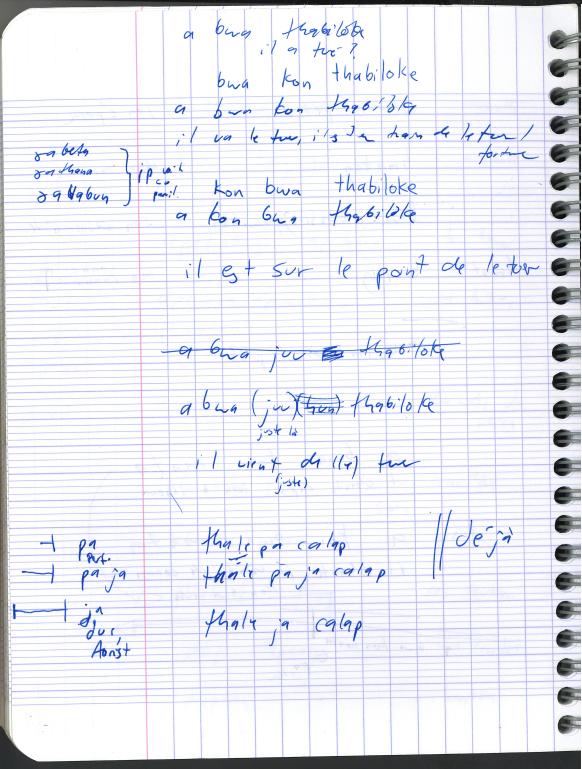
\includegraphics[width=\linewidth]{figures/vamale-170830-1005_67a}
%\label{fig:bwa_koon_notel}
%\caption{Field note extract concerning \textit{bwa koon} and \textit{koon bwa}}
%\end{figure}
%
%\begin{figure}
%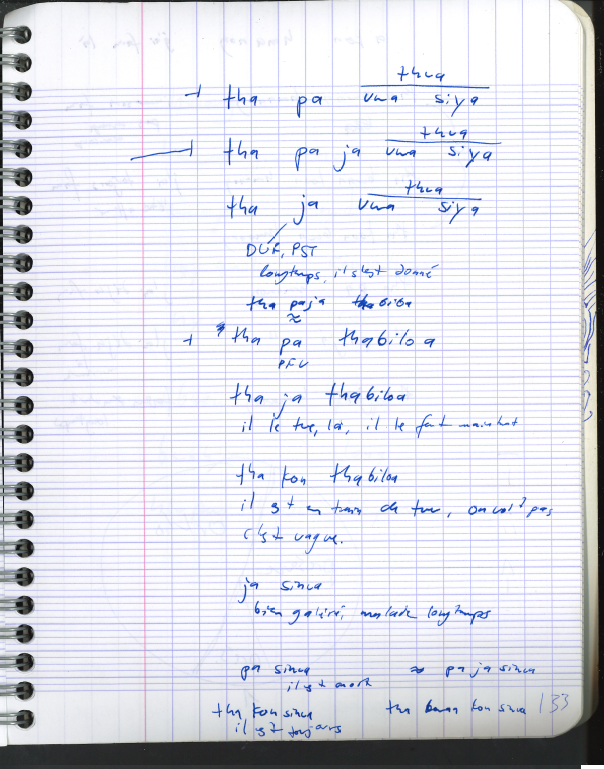
\includegraphics[width=\linewidth]{figures/vamale-170830-1005_67b}
%\label{fig:bwa_koon_noter}
%\caption{Field note extract concerning \textit{bwa koon} and \textit{koon bwa}}
%\end{figure}
%
%%todo{look at that}

 
 \section{Continuative and realis \textit{balan}}
 \label{sec:balan}
 \is{Aspect!\textit{balan}}
 
%TAM marking which uses \textit{balan} is a complex affair, because different meanings come together: continuity (despite obstacles) with durative verbs, but also realis and derived from this, immediacy to a salient moment in time.

The particle \textit{balan}, similarly to \textit{mu} described below, has more ambiguities than aktionsart can account for. Its interpretation depends on the context as well. The described event either: 

\begin{itemize}
	\item continues to happen (in some cases, despite an obstacle), 
	\item has just (unfortunately or finally) taken place or begun, 
	\item or will certainly and immediately happen.
\end{itemize}
 
\noindent The following section will first introduce \textit{balan} alone, with its two main meanings, continuative and realis, before addressing the common combinations with other aspect markers, as well as the less common ones. The section closes with a summary.
 
\textit{balan} may be a recent addition to the set of aspect markers, as speakers do not agree on the grammaticality of some of its uses, notably the combination with \textit{bo} (see \Cref{tab:balan}). One universally accepted use is that of \textit{bala-n} as a noun meaning \qu{piece of long object-\gl{nspec}}, as in \textit{balan o} \qu{piece of bamboo} and \textit{balan oot} \qu{length of string} (\ref{ex:balan_piece}). This \qu{bit} meaning allows a use of \textit{balan} as an attenuative particle, similar to \textit{xhwan}\slash\textit{xhwat} in (\ref{ex:balan_bit}) and (\ref{ex:balan_xhwan}). \is{Aspect!\textit{balan}!Attenuating}
 
 \ea
 \label{ex:balan_piece}
 % \langinfo{}{}{} 
 \gll  e=bo fe balan mwano-aen a=bo man nyako-ong\\
  1\gl{sg}=\gl{irr} take piece.length custom.cloth 3\gl{sg}=\gl{irr} rot on-1\gl{sg}.\gl{poss}\\
 \glt \qu{I'll take this piece of \textit{manou} [that you have given me as a greeting custom] and [will keep it forever so that] it will rot on me.} {[HC19:63]}
 \z
 
 
 \ea\label{ex:balan_bit}
 % \langinfo{}{}{} 
 \gll a=bo balan pala\\
  3\gl{sg}=\gl{irr} \gl{real}/bit speak\\
 \glt \qu{He will finally/a bit speak.} {[X10:55]}
 \z
 
 \ea\label{ex:balan_xhwan}
 % \langinfo{}{}{} 
 \gll a=bo xhwan pala\\
  3\gl{sg}=\gl{irr} bit speak\\
 \glt \qu{He will speak a bit.} {[X10:56]}
 \z
 
% \begin{itemize}
% 	\item balan
% 	\begin{itemize}
% 		\item a piece of a long object (\textit{wâng balan o} \qu{lit. boat piece bamboo, bamboo raft}, \textit{balan vaahit} \qu{tailless lizard [lit. bit of lizard]})
% 	\end{itemize}
% \end{itemize}

 Used as an aspect marker, \textit{balan} is more frequent in combination with other particles than alone, and \textit{balan} always comes second. A form combined with the progressive marker, \textit{kon balan}, and one with the irrealis one, \textit{bo balan} unambiguously mean \qu{has recently happened} and \qu{is just about to happen} respectively, though both are used rarely and judged ungrammatical by some speakers (especially \textit{kon balan}, perhaps because \textit{balan} expresses an immediate change of state, which contradicts \textit{kon}'s progressive meaning). Other aspectual particles precede \textit{balan} to add a sense of \qu{finally} (\textit{bwa balan}) or \qu{despite obstacles} (\textit{ja balan}). 
 
 Aktionsart also matters: durative verbs with \textit{balan} are either about to begin or have begun, but continue. Punctual verbs have either happened or are about to happen. Without context, certain verbs seem to have preferred interpretations. If the context suggests it, \textit{balan} can take an adversative function (\ref{ex:balan_adversative}). This example was elicited on the basis of a Nêlêmwa sentence with the same meaning using \textit{bara} \parencite[238]{bril_nelemwa_2002} and though the meaning \qu{unfortunately} was never found in free speech, speakers accepted it in an elicitation context.

\ea \label{ex:balan_adversative} 
\gll balan xhali sau-ng pwa-n yee	\\
 alas tear dress-1\gl{sg}.\gl{poss} on-\gl{nspec} tree	\\
\glt \qu{Unfortunately, my dress tore on a tree.}\\\relax 
[181016-jpgramm1, 00:12:56-00:12:58]
\z

\subsection{Continuative \textit{balan}}\is{Aspect!\textit{balan}!Continuative}
 Probably derived from the length-associated nominal meaning, is the aspectual use as a continuative. Used with atelic verbs, \textit{balan} can imply that the action happens despite a (potential) obstacle (\ref{ex:balan_han}), but may also refer to a lasting state (\ref{ex:balan_hmwaani}). This interpretation is only available with realis contexts, meaning that \textit{ja} \qu{\gl{prf}}, \textit{pa} \qu{\gl{prf}}, and controversial \textit{kon} \qu{\gl{prog}} are the only aspect markers that can combine with this continuative \textit{balan}. Example (\ref{ex:ja_balan}) combines \textit{balan}'s implication of an obstacle, with the resultative meaning of \textit{ja} to imply an expected hurdle. This is discussed in more detail in \sectref{ssec:ja_balan}. \textit{balan} is also found in the verb \textit{fe balan} \qu{to continue (lit. take length)}, and as an adverb meaning \qu{ever since}, see (\ref{ex:balan_since}).
 

 \ea\label{ex:balan_han}
 % \langinfo{}{}{} 
 \gll e=balan han\\
  1\gl{sg}=\gl{cont} walk\\
 \glt \qu{I keep walking (despite e.g. your calling me).} {[J2:39]}
 \z
 
 
 \ea\label{ex:balan_hmwaani}
 % \langinfo{}{}{} 
 \gll na i=s-ung tha balan hmwaani\\
  \gl{dem} \gl{def}.\gl{sg}=hand-1\gl{sg}.\gl{poss} \gl{ass} \gl{cont} like.this\\
 \glt \qu{It's my arm, it stays like this.} {[KG:139]}
 \z
 
 \ea\label{ex:ja_balan}
 % \langinfo{}{}{} 
 \gll e=ja balan jili wâng\\
  1\gl{sg}=\gl{prf} \gl{cont} build boat\\
 \glt \qu{Despite an expected holdup, I keep boat-building.} {[J2:43]}
 \z
 
 
 \ea\label{ex:balan_since}
 % \langinfo{}{}{} 
 \gll balan cel=e=xale-ko\\
  since when.\gl{real}=1\gl{sg}=see-2\gl{sg}.\gl{obj}\\
 \glt \qu{ever since I saw you} {[example sentence for the dictionary]}
 \z

 
 \subsection{Realis \textit{balan}}
 \is{Aspect!\textit{balan}!Realis}
 In irrealis situations, with punctual or telic verbs, and with atelic ones in the appropriate pragmatic context, \textit{balan} means something completely different: the realization of a situation.\footnote{Durative verbs do not carry the meaning \qu{just done}, but rather \qu{recently started and continuing}.} The continuative meaning discussed above maintains a situation, whereas this realis sense is concerned with change. With meanings ranging from \qu{this has just begun/come to happen} to \qu{finally}, the common denominator of non-continuative \textit{balan} is that the resulting construction is a realis one, or is so close to becoming one that it might as well already be. This is the reason why \textit{bo balan} is contested (see \sectref{ssec:bo balan}); it seems to be more widely accepted by younger speakers. \textit{bwa balan} ambiguously means either \qu{has recently begun and is still underway} and \qu{has practically begun}, probably both using the ambiguity of \textit{bwa} as both a realis and irrealis marker (\ref{sec:bwa}), and at least originally coming from hyperbole (\qu{I'm so close to doing it that I've practically begun}). However, neither of these explanations would work with \textit{bo}, which is explicitly irrealis and thus unlikely to be used here for hyperbole, as well as being unavailable for combinations with realis markers. The use of \textit{bo} with \textit{balan}, shown with its ambiguous meanings in  (\ref{ex:bo_balan}), may point at a development of \textit{balan} towards a more flexible meaning. %as in it's less striclty realis and more focused on the immediacy of limits 
 Interestingly, the ambiguity that \textit{balan} can express with regard to conceptual limits is shared by \textit{xhwan} \qu{almost, hardly}, and not unknown in other languages of the area (e.g. \textit{(k)u} \qu{\gl{prf}}, \citealt[206, 207]{bril_nelemwa_2002}). 
 
% A border close to the temporal reference point (almost finished/only just started?). There seems to be an ambiguity with durative verbs (\qu{a little bit}, see \ref{sec:bwa_balan} "bamboo raft"), but maybe this is a mistake of mine.

\begin{table}
	\caption{Overview of aspect marker combinations with \textit{balan}}
	\begin{tabularx}{\textwidth}{QQQQl}
	\lsptoprule
		\multicolumn{5}{c}{subject marker= \textit{b.}= verb}\\
		\textit{balan} & \textit{ja b.} & \textit{bwa b.} & \textit{kon b.} & \textit{bo b.}\\\midrule
		just done\slash about to do, continue to do, do despite  & finally do, do despite constraints & finally do (but not \textit{despite})& just begun\slash about to do & about to do\\
		\lspbottomrule
	\end{tabularx}
	\label{tab:balan}
\end{table}

\ea \label{ex:bo_balan} 
\gll gase=bo balan hmasan!\\
 1\gl{pl}.\gl{incl}=\gl{irr} \gl{real} bit arrive\\
\glt \qu{We will finally arrive!} {[X10:54]}
\z

\ea 
\gll a=bo balan pala\\
 3\gl{sg}=\gl{fut} \gl{real}/\gl{prf} speak\\
\glt \qu{He will finally/a bit speak.} {[X10:55]}
\z

\subsection{Finally, continuative: \textit{ja balan}}
\label{ssec:ja_balan}
\is{Aspect!\textit{balan}!Continuative}\is{Aspect!\textit{balan}!Realis}
The combination of \textit{ja} \qu{\gl{prf}} and \textit{balan} shows the oft-encountered temporal immediacy due to \textit{balan}, but \textit{ja}'s contribution is less clear. In examples (\ref{ex:jab1}) and (\ref{ex:jab2}), the meaning \qu{finally} is derived from \textit{ja}. In (\ref{ex:jab3}), \textit{balan} marks perseverance despite an obstacle, and \textit{ja} seems to mark that the obstacle is one that was known beforehand, perhaps relating to single \textit{ja}'s meaning of \qu{finally, after an observed period of becoming}.% (but keep in mind that \textit{balan} as a noun means \qu{a length of something}).

%\begin{table}
%	\caption{\textit{ja} balan}
%	\begin{tabular}{lllll}
%		aktionsart& word & before & \multicolumn{2}{c}{after}\\
%		\hline&&&&\\
%		\multirow{4}{1cm}{punctual}&arrive & about to & &just done\\
%		& finish & &done \emph{anyway}& \\
%		& die & & done \emph{anyway} &\\
%		&speak & finally & \emph{continue} to & \\
%		&&&&\\
%		\hline &&&&\\
%		\multirow{3}{1cm}{durative} &walk & & continue to &\\
%		&read & & & just begun, still happening\\
%		&build	&	& continue to &\\
%	\end{tabular}
%\end{table}

\ea\label{ex:jab1}
\gll a=ja balan pala\\
 3\gl{sg}=\gl{prf} \gl{cont} speak\\
\glt \qu{He continues to speak, he will finally speak.}\\
% \qu{Il continue à parler, il va parler}
\z


\ea\label{ex:jab2}
\gll 	e=ja balan fine i=tii	\\
	1\gl{sg}=\gl{prf} \gl{cont} read \gl{def}.\gl{sg}=book	\\
\glt	\qu{You (will) finally begin to read the book.}%\qu{T'as commencé à lire le livre.} \\ \qu{je suis sur le point de lire}	
\z


\ea
\gll gase={ja} balan hmasan!\\
 1\gl{pl}.\gl{incl}=\gl{prf} \gl{cont} arrive\\
\glt \qu{We are finally about to arrive, we have just arrived!}
%\qu{On est sur le point d'arriver, on vient d'arriver}
\z


An adversative meaning is not only achieved with \textit{balan} alone (\ref{ex:balan_adversative}), but also in combination with \textit{ja} \qu{\gl{prf}} (\ref{ex:ja_balan}). The meaning added to the simple adversative is one of foresight: the obstacle against which the predicate takes place is an expected one.

\ea
\gll e=ja balan han\\
 1\gl{sg}=\gl{prf} b. go\\
\glt \qu{I went on [despite my scheduled meeting].}
\z

\ea\label{ex:jab3} 
\gll 	e=ja balan jili wâng	\\
	1\gl{sg}=\gl{prf} b. build boat	\\
\glt \qu{I continue building my boat despite X.} {[J2:43]}%	\qu{Je continue à construire mon bateau (malgré des imprévus)}	
\z

\subsection{Finally: \textit{bwa balan}}
\label{sec:bwa_balan}
\is{Aspect!\textit{balan}!Realis}
\textit{bwa balan} marks an immediate temporal limit. For punctual verbs, this means either a recent end (\ref{ex:balanfinally}) or a recent beginning (\ref{ex:balanconv1}). For durative verbs, \textit{bwa balan} implies ongoing action (\ref{ex:balanconv2}). This is by far the most frequent form with \textit{balan}. \Cref{tab:bwabalan} summarizes the meanings with different verbs. 

\begin{table}
	\caption{bwa \textit{balan}}
	\begin{tabular}{llll}
	\lsptoprule
		Aktionsart& verb & future meaning & past\slash progressive meaning \\\midrule
		punctual&arrive & &recently done\\
		&finish & & recently done\\
		%	& die & & finally done? \\
		durative	&speak & about to& recently begun, \textit{still happening}  \\
		 &walk & about to  &recently begun, \textit{still happening}\\
		&read & & recently begun, \textit{still happening}\\
		&build	&	&  recently begun, \textit{still happening}\\
	\lspbottomrule
	\end{tabular}
\label{tab:bwabalan}
\end{table}


\ea\label{ex:balanfinally}
\gll gase={bwa} balan hmasan!\\
 1\gl{pl}.\gl{incl}=\gl{ipfv} bit arrive\\
\glt \qu{We finally arrived recently; we are about to finally arrive (this is so sure and immediate that we might as well have already arrived)!}%\qu{on est arrivé récemment}
\z

\ea\label{ex:balanconv1}
\gll e=bwa balan han\\
 1\gl{sg}=\gl{ipfv} b. go\\
\glt \qu{I am (finally about to be) leaving.}
\z

\ea\label{ex:balanconv2}
\gll 	e=bwa balan fine i=tii	\\
	1\gl{sg}=\gl{ipfv} b. read \gl{def}.\gl{sg}=book	\\
\glt	\qu{I have finally begun reading.}%\qu{J'ai commencé à lire}	
\z

While some verbs have a conventional interpretation, such as telic (\ref{ex:balanconv1}) and atelic (\ref{ex:balanconv2}), ambiguous, context-dependent cases are common (\ref{ex:balan_imm}), possibly because \textit{bwa} has many possible interpretations. %The combination \textit{bwa balan} is an example of the influence of the modified verb's aktionsart on TAM marker meaning.

\ea \label{ex:balan_imm}
\gll 	e=bwa balan jili wâng	\\
	1\gl{sg}=\gl{ipfv} b. build boat\\
\glt	\qu{I will begin building the boat (this is so sure that I have practically begun); I have begun.}%\qu{Je commence à construire le bateau, j'ai commencé}	
\z

\ea 
\gll a=bwa balan pala\\
 3\gl{sg}=\gl{ipfv} b. speak\\
\glt \qu{He has just spoken; he has begun to speak.} {[X10:51]}
\z
  %\todo{are the latter two not \textit{bwa balan}}


%However, the meaning is not completely up to its pragmatic context. Compare  (\ref{ex:bwa_balan_vi}) and (\ref{ex:bwa_vi}), repeated below: in both cases, a temporal border is close to the moment of speech. However, the reason why \textit{balan} makes the situation a past one in (\ref{ex:bwa_balan_vi}) is unclear. \textit{balan} probably contributes the notion of \qu{finally}, and \textit{bwa} possibly the meaning that it is close to the moment of speech.  %As \textit{vi} is durative, a future meaning of \textit{bwa} is not the only possibility. 
%
%\ea
%\ea\label{ex:bwa_balan_vi}
%
%\langinfo{}{}{} X10:50
%\gll e=bwa balan vi nyakoo-n
% 1\gl{sg} \gl{ipfv} \gl{cont} say \gl{obl}-3\gl{sg}.\gl{poss}
%\glt \qu{I have finally told him}
%
%
%\ea\label{ex:bwa_vi2}
%
%\langinfo{}{}{} X10:49
%\gll e=bwa vi nyakoo-n
% 1\gl{sg} \gl{ipfv} say \gl{obl}-3\gl{sg}.\gl{poss}
%\glt \qu{I will tell him}
%
%\z 
%Pragmatic context is important: comparing telic \textit{thabiloke} \qu{to kill} in (\ref{ex:bwa_balan-kill}) to atelic \textit{pala} \qu{talk} in (\ref{ex:bwa_balan-speak}), it appears that the telic verb is an action which finally happened, whereas with an atelic verb, a simple recent past is expressed. 
%
%\ea
%\ea\label{ex:bwa_balan-kill}
%
%\langinfo{}{}{} JR:17.8
%\gll ka e=bwa balan tha-bilo-a\textsuperscript{telic}
% \gl{cnj} 1\gl{sg} \gl{ipfv} b. with.strike-kill-3\gl{sg}.\gl{obj}
%\glt \qu{And finally I killed him.}
%
%\ea \label{ex:bwa_balan-speak}
%
%\langinfo{}{}{} X10:51
%\gll e=bwa balan pala\textsuperscript{atelic}
% 1\gl{sg} \gl{ipfv} b. speak
%\glt \qu{I have just spoken (I spoke very recently)}
%
%\z

\subsection{\textit{kon balan} \qu{about to, recently started}}
\is{Aspect!\textit{balan}!Realis}
Few speakers accept this form without context. If one needs to make clear that something has begun and is going on, this may be possible (\ref{ex:konb1}). Punctual verbs are even more contested, likely because of the progressive \textit{kon}.

\begin{table}
	\caption{kon \textit{balan}}
	\begin{tabular}{llll}
	\lsptoprule
		Aktionsart&Gloss of form & &\\\midrule
		\gl{punc}&arrive & &recently done\\
		&speak & \textit{finally} about to&  \\\addlinespace
		\gl{dur} &walk & \textit{finally} about to &  \\
		&read & &  recently begun\\
		&build	& &recently begun \\
	\lspbottomrule
	\end{tabular}
	\label{tab:kon_balan}
\end{table}

\ea
\gll 	e=kon balan jili wâng	\\
	1\gl{sg}=\gl{prog} \gl{real} build boat	\\
\glt	\qu{I have begun building the boat.}	
\z

\ea\label{ex:konb1}
\gll 	e=kon balan fine i=tii	\\
	1\gl{sg}=\gl{prog} \gl{cont} read \gl{def}.\gl{sg}=book	\\
\glt	\qu{(rare) I continue reading the book (it has just begun).}%\qu{(rare) Je continue à lire le livre}	
\z	

\subsection{\textit{bo balan} \qu{about to}}
\label{ssec:bo balan}
\is{Aspect!\textit{balan}!Realis}
The combination of \textit{bo} with \textit{balan} is not accepted by many older speakers, and is mostly used to unambiguously state on which side of the temporal border we are: the event is about to happen (\ref{ex:bobalan1}, \ref{ex:bobalan2}). One speaker translated an example with a realis meaning (\ref{ex:bobalan3}), but none were produced spontaneously.
%\begin{table}
%	\centering
%	\caption{bo \textit{balan}}
%	\begin{tabular}{llll}
%		punctual&arrive & \textit{finally} about to  &\\
%		& finish & & about to \\
%		& die & * & *   \\
%		&speak & \textit{finally} about to &  \\
%		&leave & \textit{finally} about to &  \\ &&&&\\
%		%durative	&read & & & recently begun, \textit{still happening}\\
%	durative	&build	& about to	& \\
%	\end{tabular}
%\end{table}

%A troubling detail is the meaning of durative \qu{fine} \qu{read, count}. The fact that an irrealis marker \textit{bo} can be interpreted as something realis is found nowhere else in the language. A tentative explanation would be that \textit{bo balan} is contested anyway, and that this confusing reading of it is due to the elicitation setting and the contrived nature of data collection.



	\ea\label{ex:bobalan1}
	[,am.bom.ba.lan.'pa.la]\\
	\gll a=bo balan pala\\
	 3\gl{sg}=\gl{irr} bit speak\\
	\glt \qu{He will finally speak.} {[X10:55]}
	\z
	
	\ea\label{ex:bobalan2}
	% \langinfo{}{}{} 
	%\langinfo{}{}{} 2017-09-01 Kito Nigai Thea
	\gll gase=bo balan hma-san!\\
	 1\gl{pl}.\gl{incl}=\gl{irr} \gl{prf} arrive-same.level\\
	\glt \qu{We will finally arrive!} {[X10:54]}
	\z
	
%	\a
%	
%	\langinfo{}{}{} [,em.bom.ba.'lan.hãn]
%	\gll e=\textbf{bo} balan han
%	 1\gl{sg} \gl{irr} \gl{cont} go
%	\glt \qu{I go on.}
%	
	
	\ea\label{ex:bobalan3}
	% \langinfo{}{}{} 
	\gll 	e=bo balan jili wâng	\\
		1\gl{sg}=\gl{irr} \gl{real} build boat	\\
	\glt	\qu{I begin building.} {[J2:44]}
	%\qu{Je commence à construire...}
	\z



 
\subsection{Summary: Combinations with \textit{balan}}
 While the chapter features a summarizing table at the end (\Cref{tab:aspect_combo}), % and this section an own table for \textit{balan} (\Cref{tab:balan_combo}), 
the following examples summarize the various functions of \textit{balan}. The data below were elicited explicitly as minimal examples and may present an over-simplified view. %, though the preceding section ``\sectref{sec:balan}" has done its best to muddle any convictions.
 
 \ea
 \gll 	e=fine i=tii	\\
 	1\gl{sg}=read \gl{def}.\gl{sg}=book	\\
 \glt	\qu{I read the book.}
 \z
 
 \ea
 \gll 	e=balan fine i=tii	\\
 	1\gl{sg}=\gl{real} read \gl{def}.\gl{sg}=book	\\
 \glt \qu{I just started reading a book, I am still reading it.}	%\qu{Trouvé un livre et tu lis tout de suite}	
 \z
 
 \ea
 \gll 	e=kon balan fine i=tii	\\
 	1\gl{sg}=\gl{prog} \gl{cont} read \gl{def}.\gl{sg}=book	\\
 \glt	\qu{(rare) I continue reading the book (it has just begun).}%\qu{(rare) Je continue à lire le livre}	
 \z
 
 \ea
 \gll 	e=bwa balan koin fine i=tii	\\
 	1\gl{sg}=\gl{ipfv} \gl{real} finish read \gl{def}.\gl{sg}=book	\\
 \glt	\qu{I have finished reading the book (just now).}%\qu{J'ai bien fini de lire}	
 \z

 \ea
 \gll e=bo balan koin fine i=tii\\ 
  1\gl{sg}=\gl{irr} \gl{real} finish read \gl{def}.\gl{sg}=book	\\
 \glt \qu{I am about to finish reading the book.}
 % \a
% 
% \gll 	e bwa koin fine i tii	
% 	1\gl{sg} \gl{ipfv} finish read \gl{def}.\gl{sg}=book	
% \glt	\qu{I am interrupting my reading (lit. I am stopping reading the book)}%\qu{Je m'arrête de lire (pour un moment)}	
% 
 \z
 
 Missing from this collection of examples is \textit{ja balan} \qu{finally \textit{balan}}, because the pragmatic context is so important that a representative example is impossible. 
 
%\begin{table}
% 
% 	\caption{Combinations with \textit{balan}: \textit{ja} \gl{prf}}
% 	\begin{tabularx}{\linewidth}{l|ll}
% 		\multicolumn{3}{c}{subject marker  \textit{balan}  verb}\\
% 		\hline &&\\
% 		verb & \textit{balan} & \textit{\textbf{ja} b.}\\
% 		&&\\
% 		\hline&&\\
% 		&just done / about to do  & do after long struggle, do/ \\
% 		&&achieve despite constraints\\
% 		\hline&&\\
% 		\textit{hma koon} \qu{find}& about to / just happened& \textbf{finally/despite X}: about to / just happened\\
% 		\textit{hmasan} \qu{arrive}& about to / just happened& \textbf{finally/despite X}: about to / just happened\\
% 		\textit{koin} \qu{end}& about to / just happened& \textbf{finally/despite X}: about to / just happened\\
% 		\textit{me} \qu{die}& about to / just happened& \textbf{finally/despite X}: about to / just happened\\
% 		\textit{pala} \qu{talk}& about to / still going& \textbf{finally/despite X}: about to / just happened\\
% 		\textit{han} \qu{go}& about to / still going& \textbf{finally/despite X}: about to / just happened\\
% 		\textit{fine} \qu{read}&about to / still going& \textbf{finally/despite X}: about to / just happened\\
% 		\textit{jili} \qu{build w/ wood}& about to / still going& \textbf{finally/despite X}: about to / just happened\\
% 	\end{tabularx}
% 	\label{tab:balan_combo}
%\end{table}

%\begin{table}
% \caption{Combinations with \textit{balan}: \textit{bwa} \gl{ipfv}, \textit{bo} \gl{fut}, \textit{kon} \gl{prog}}
% \begin{tabularx}{\linewidth}{l|lll}
% 	\multicolumn{4}{c}{subject marker  \textit{balan}  verb}\\
% 	\hline &&&\\
% 	verb & \textit{\textbf{bwa} b.} &  \textit{bo b.} & \textit{kon b.}  \\
% 	&&&\\
% 	\hline&&&\\
% 	& \textbf{finally} do /done & about to do & has just happened\\
% 	\hline&&&\\
% 	\textit{hma koon} \qu{find}&  \textbf{finally}: about to / just happened& about to& just now happened\\
% 	\textit{hmasan} \qu{arrive}& \textbf{finally}: about to / just happened&about to&just now happened\\
% 	\textit{koin} \qu{end}&  \textbf{finally}: about to / just happened&about to&just now happened\\
% 	\textit{me} \qu{die}& \textbf{finally}: about to / just happened&about to&just now happened\\
% 	\textit{pala} \qu{talk}&\textbf{finally}: about to / just happened&about to&just now happened\\
% 	\textit{han} \qu{go}& \textbf{finally}: about to / just happened&about to&just now happened\\
% 	\textit{fine} \qu{read}& \textbf{finally}: about to / just happened&about to&just now happened\\
% 	\textit{jili} \qu{build w/ wood} &\textbf{finally}: about to / just happened&about to&just now happened\\
% \end{tabularx}
% \label{tab:balan_combo2}
%\end{table}
 
 \section{Perfective \textit{pa (ja)} }
  \label{sec:pa ja}
  
The perfective marker \textit{pa}, marks the predicate as completed by the moment of speech (\ref{ex:pa}), or the relative temporal reference point, e.g. in stories. 

\ea \label{ex:pa} 
\gll cama=a=vi hapi a=pa xhwi-aman\\
 if=3\gl{sg}=say \gl{comp} 3\gl{sg}=\gl{prf} eat-thing\\
\glt \qu{If he says that he's already eaten [stop trying to feed him].} {[D3:78]}
\z

Contrary to most other aspectual markers, \textit{pa} is indifferent to aktionsart. \textit{pa} with an atelic verb means that this has already begun or finished depending on the context, and with a telic verb, that it has taken place. It is commonly translated as \textit{déjà} \qu{already} in French and stylistically often used in this sense. 
 
 Associating \textit{pa} with \textit{ja} \qu{\gl{prf}} (see \sectref{sec:ja}) adds the information that the completion took some time, or was long awaited, as in (\ref{ex:pa_ja1}), or that whatever is marked has happened some time ago, as in (\ref{ex:pa_ja2}). This is by far the most common combination with \textit{pa}.
 

 \ea \label{ex:pa_ja1}
 %\langinfo{}{}{}  
 \gll le=ja vatipwe-mwa kon ya tha pa ja me-a go tha le=ja thuat-mwa moo ka li=xhaomu ja tha le=ja ha-mwa-me \\
  3\gl{pl}=\gl{prf} drop-\gl{rep} because 3\gl{sg} \gl{ass} \gl{prf} \gl{prf} die-3\gl{sg} then \gl{ass} 3\gl{pl}=\gl{prf} emerge-\gl{rep} stay \gl{sbj} \gl{def}.\gl{pl}=elder \gl{prf} \gl{ass} 3\gl{pl}=\gl{prf} go-\gl{rep}-\gl{dir.cp}\\
 \glt  \qu{They were released [again] because he was already dead, and they came out of prison [again] and came back.} {[HC1:32]}
  \z
 
 
 \ea\label{ex:pa_ja2}
 \gll ma le=ta ma le=xale-a koma le=fe-a ma le=ta ma le=fe-a, ya pa ja me-a  \\
  \gl{com} 3\gl{pl}=go.up \gl{com} 3\gl{pl}=see-3\gl{sg} so.that 3\gl{pl}=take-3\gl{sg} \gl{com} 3\gl{pl}=go.up \gl{subr} 3\gl{pl}=take-3\gl{sg} 3\gl{sg} \gl{prf} \gl{prf} die-3\gl{sg} \\
\glt \qu{And they went up, saw him, in order to catch him, they went up to catch him, he (however) was already dead.} {[HC1:29]} 
 \z

As illustrated in (\ref{ex:paja_cipe}), \textit{pa} (with its frequent companion \textit{ja}) can precede the subject index, though this is rare. This is also attested for \textit{bwa} \qu{\gl{ipfv}}; both are only found in negated contexts. The semantic difference achieved, like with \textit{bwa}, is that \textit{cipe pa ja jili bwaakala} \qu{I don't already build boats} does not clarify whether the subject ever built boats, whereas \textit{pa ja} in the first position adds a sense of achievement to the statement \qu{I don't build boats}, i.e. \qu{my building days are done}.

\ea \label{ex:paja_cipe}
\gll pa ja cip=e jili bwaakala\\
 \gl{prf} \gl{prf} \gl{neg}=1\gl{sg} build.with.wood outrigger.canoe\\
\glt \qu{I already don't build boats anymore.} [B2:144]
\z

\section{Perfect \textit{ja} \qu{finally}}
\label{sec:ja}
\is{Aspect!\textit{ja} \qu{finally}}
The Bwatoo cognate of this form, \textit{je}, is glossed as ``accomplished" \parencite[56]{rivierre_bwatoo_2006}. For atelic verbs, \textit{ja} expresses the expected, or long-awaited beginning of the action, as in (\ref{ex:ja_hantabo}), (\ref{ex:ja_hup}), and (\ref{ex:ja_seada}). Note the verb \textit{jake} \qu{measure, weigh}, which may be related.


\ea\label{ex:ja_hantabo}
\gll ...hê a={ja} han tabo pwan bwa-n, koin a={ja} fe-ta-mwa-me-a\\
 yes 3\gl{sg}=\gl{prf} go sit on head-3\gl{sg}.\gl{poss} then 3\gl{sg}=\gl{prf} take-go.up-\gl{rep}-\gl{dir.cp}-3\gl{sg}.\gl{obj}\\
\glt \qu{Yes, he\textsubscript{i} eagerly climbs to sit on his\textsubscript{ii} head, then he\textsubscript{ii} takes him\textsubscript{i} home.} {[HC2:26] (see \Cref{text:squid2})}
\z

%\ea
%
%\langinfo{}{}{} HC2:27-28 (context for following)
%\gll ...lu hmaca-mwa-me can hmeewan, ma xhasat nyada-mwa siibwi phwâêû.
% 3\gl{du} arrive-\gl{rep}-\gl{dir.cp} in sand \gl{com} jump send-\gl{rep} rat dry.land 
%\glt \qu{The two arrive on the beach and the rat jumps unto dry land.}
%

\ea\label{ex:ja_hup}
\gll go cama i=ibwen a={ja} hup- a=kon {ja} hup-wa-e can we...\\
 then concerning \gl{def}.\gl{sg}=squid 3\gl{sg}=\gl{prf} go.down 3\gl{sg}=\gl{prog} \gl{prf} go.down-\gl{rep}-\gl{dir.cf} in water\\
\glt \qu{Then, when the squid finally goes down back into the water\ldots}\\ \qu{Then, once the squid had gone back into the water [and the rat thought himself at a safe distance to mock him]...} {[HC2:29]}
\z

\ea \label{ex:ja_seada}
\gll siibwi tha pa me-a. tha=a=pa {ja} sea-da\\
 rat \gl{ass} \gl{prf} die-3\gl{sg} \gl{ass}=3\gl{sg}=\gl{prf} \gl{prf} gaze-up \\
\glt \qu{The rat is dead. He ended up gazing upwards.} {[HC2:40]}
\z

\ea \label{ex:ja_end}
\gll cama ibwen tha=a={ja} hup-wa, tha ja koin mwa \\ %\textsuperscript{temp. deix}
 concerning squid \gl{ass}=3\gl{sg}=\gl{prf} go.down-\gl{rep} \gl{ass} \gl{prf} end \gl{rep}\\
\glt \qu{And the squid, he went back down. This is the end.}\\
\qu{The squid has gone down, thus it has ended.} {[HC2:39-40]}
\z

With telic verbs, \textit{ja} marks that something finally happens, be it that it was actively anticipated (\textit{tha jaa koin} \qu{it's finally over}) or (\ref{ex:ja_vwa}), or that it was expected and inevitable like one's own departure from a social situation: \textit{e bwaa ja han} \qu{I'm about to finally leave}. The latter function likens it to \textit{pa} (\sectref{sec:pa ja}), with which it often associates. Whereas \textit{pa} only marks that the action is completed by the temporal point of reference, \textit{ja} adds a sense of \qu{finally}, similar to Comrie's ``perfect of result" \parencite[58]{comrie_aspect_1981}. This also applies to the result of a natural process: \textit{bwaam, tha jaa xhopwe-go!} \qu{My, you've grown!}. Stylistically, \textit{ja} may to be used to close a scene, see (\ref{ex:ja_end}) and Swamp Hen's takeoff (\ref{ex:ja_ta}, \ref{ex:ja_ta2}), where \textit{ja} marks the final leave of the swamp hen; we do not see her again. It cannot be used to describe the death of a person, as this would suggest that their death was expected. Given that \textit{ja} expresses the result of an observed process and introduces a situation that is relevant for the time of reference (the present in direct situations, the narrative time in stories), \textit{ja} will be labelled as ``perfect". 

%Means that whatever follows is now over, does not occur alone to describe present situations
%Telic:

\ea\label{ex:ja_vwa}
\gll ...go a={ja} vwa mwa me ka i=siibwi.\\
 then 3\gl{sg}=\gl{prf} do \gl{rep} die \gl{sbj} \gl{def}.\gl{sg}=rat\\
\glt \qu{Then he killed him.} {[HC2:38]}% ("il l'a tué")}
\z 

\ea\label{ex:ja_ta}
\gll go tha=a={ja} ta-mwa-me\\
 then \gl{ass}=3\gl{sg}=\gl{prf} go.up-\gl{rep}-\gl{dir.cp}\\
\glt \qu{And then it went home.} {[HC2:12]} 
\z

\ea\label{ex:ja_ta2}
\gll ya tha {ja} thêên thêên ta-mwa-me\\
 3\gl{sg} \gl{ass} \gl{prf} fly fly go.up-\gl{rep}-\gl{dir.cp}\\
\glt \qu{Flew home right away.} {[HC2:13]} 
\z

\section{Present perfective \textit{kon ja}}
In combination with \textit{kon} \qu{\gl{prog}}, \textit{ja} expresses something that is done by the moment which \textit{kon} designates (\ref{ex:konja}). 

\ea \label{ex:konja}
\gll putain yo m=e th=e=kon ja vwa i=\textit{signe}\\
 fuck 1\gl{sg} \gl{subr}=1\gl{sg} \gl{ass}=1\gl{sg}=\gl{prog} \gl{prf} do \gl{def}.\gl{sg}=sign\\
\glt \qu{Rats, I should have given [him] a sign by then.} {[KG:492]}
\z 
%\ea 
%\ea
%
%\langinfo{}{}{} Fable of the North Wind and the Sun, V1:4
%\gll ka i wabataan a \textbf{ja} juu cika mwa\textsuperscript{anymore?} wîîn
% \gl{cntr} \gl{def}.\gl{sg}=north.wind 3\gl{sg} \gl{prf} really \gl{neg}.\gl{exist} \gl{rep} strength
%\glt \qu{And the North Wind had no strength left.}
%
%
%\a
%
%\langinfo{}{}{} V1:5 (for context)
%\gll ka i xat a bwa nyoot mwa\textsuperscript{temp. deix?} nya wîîn
%  \gl{cntr} \gl{def}.\gl{sg}=sun 3\gl{sg} \gl{ipfv} come.out \gl{rep} give strength
%\glt \qu{And the Sun shone strongly}
% 
%
%\a
% 
%\langinfo{}{}{} V1:5 (for context)
%\gll ka i apuli a \textbf{ja} juu uti saun
%  \gl{cntr} \gl{def}.\gl{sg}=man 3\gl{sg} \gl{prf} really take.off cloak   
%\glt \qu{And the man took off his cloak immediately.}
% 
%\z
 
 \section{Frequentative and iterative \textit{mu}}
  \label{sec:mu}	
 \textit{mu} is a versatile particle, and can mean \qu{as well; all along, during a certain time; at selected moments over a long period of time}. \is{Aspect!Frequentative \textit{mu}}Depending on the aktionsart and the aspectual context of the verb, \textit{mu} can take on frequentative functions (\ref{ex:mu_freq}): this concerns telic verbs in general (\ref{ex:mu_aube_tel} and \ref{ex:mu_taemwi}), and countable, finished events (\ref{ex:mu_bwa1} and \ref{ex:muoften1}).% \textit{mu} reacts not only to telicity. An atelic event can have happened all along over a period of time, or, if the context is understood to be present instead of past, the atelic event is happening as we speak, little by little.
 
% \ea
 \ea\label{ex:mu_aube_tel}\label{ex:mu_freq}
 \gll m=e xa-vwa hmwata i=bee-ng a=mu xhajake\\
  \gl{irr}=1\gl{sg} \gl{hab}-make starchy.cake \gl{def}=brother-1\gl{sg}.\gl{poss} 3\gl{sg}=\gl{freq} eat.starchy\\
 \glt \qu{Whenever I make a yam cake, my brother eats it.} {[X10:40]}
  \z
 
 \ea\label{ex:mu_taemwi}
 \gll calibeen goakan e=mu taemwi li=nyu \\
  sometimes moment 1\gl{sg}=\gl{freq} catch \gl{def}.\gl{pl}=fish\\
 \glt \qu{I catch fish every time.} {[X10:42]}
 \ex\label{ex:mu_bwa1}
 \gll e=bwa mu majit\\
  1\gl{sg}=\gl{ipfv} \gl{freq} rest\\
 \glt \qu{I sleep from time to time.} {[J4:31]}
 \ex\label{ex:muoften1}
 \gll ca i=nyan-mwa xahan le=mu sivu sikaa \\
  in \gl{def}.\gl{sg}=inside-house  over.there 3\gl{pl}=\gl{freq} blow cigarette \\
 \glt \qu{They have the habit of smoking in this room over there.} {[X10:44]}
 \z
 \is{Aspect!Iterative \textit{mu}}
 Another function is iterative, with durative verbs (\ref{ex:mu_it}). There is a difference in meaning with past and present situations, i.e. an ongoing action with \textit{mu} is yet incomplete and evolving bit by bit (\ref{ex:mu}), whereas a past action happened several times or bit by bit (\ref{ex:mu_bwa2}). With a stative verb (\ref{ex:muxhwatin}), it may mean a development, as with \textit{e-} \qu{\gl{mid}} (\sectref{ssec:MID_unbounded}).
 
% \ea
 \ea\label{ex:mu}\label{ex:mu_it}

 \gll a=mu hnuut\\
  3\gl{sg}=\gl{iter} go.downstream\\
 \glt \qu{He is (still) going down.} {[J4:27]}
 \ex\label{ex:mu_bwa2}
 \gll e=bwa mu tena ha-mwa\\
  1\gl{sg}=\gl{ipfv} \gl{iter} hear go-\gl{rep}\\
 \glt \qu{I heard about it all along.} {[Tipije]}
 \ex \label{ex:muxhwatin}
 %\langinfo{}{}{} \textit{mu}, an iterative marker for durative verbs
 % vamale-180929-ddgrammaire-04 00:40:55 -- 00:41:46
 \gll 	a=mu xhwatin	\\
 	3\gl{sg}=\gl{iter} small	\\
 \glt	\qu{It is shrinking.}	
 \z
  
However, \textit{mu} can also have additive meanings (for states, as in (\ref{ex:mu_too})). Note that this is only attested in combination with \textit{pa} \qu{already}.\is{Aspect!Additive \textit{mu}}\largerpage
%\label{ex:mu_add}
	\ea\label{ex:mu_too}\label{ex:mu_add}
	\gll tha pa mu hman-ong\\
	 \gl{ass} already \gl{add} hungry-1\gl{sg}\\
	\glt \qu{I, too, am hungry already.} {[J4:30]}
	\ex\label{ex:mu_as-well}
	\gll e=paa mu majit\\
	 1\gl{sg}=\gl{prf} \gl{add} rest\\
	\glt \qu{I, too, am already asleep.} {[J4:32]}
	\z

Some uses are ambiguous, with durative, atelic verbs that can be understood as countable events (\ref{ex:muoften2}). The meanings of \textit{mu} are summarized in \Cref{tab:mu}.
 \ea \label{ex:muoften2}
\gll e=mu se\\
 1\gl{sg}=\gl{iter}/\gl{freq} cry\\
\glt \qu{I cry (often; still).} {[X10:92]}
\z


\begin{table}
	\centering
	\caption{Shades of \textit{mu}}
	\begin{tabularx}{\textwidth}{llQl}
		\lsptoprule
		& \textit{mu} & \textit{bwa mu} & \textit{pa mu} \\
		\midrule
		atelic  &  still, every time (\ref{ex:muoften1}, \ref{ex:muoften2}) & several times over time (opt. with \textit{hamwa}) (\ref{ex:mu_bwa1}, \ref{ex:mu_bwa2})     &  also (\ref{ex:mu_add}) \\
		telic  & every time (\ref{ex:mu_aube_tel})&     \\
\lspbottomrule
	\end{tabularx}
	\label{tab:mu}
\end{table}


%\begin{table}[]
%	\centering
%	\caption{My captionxx}
%	
%	\begin{tabular}{lllll}
%		& \multicolumn{2}{c}{mu}      & pa mu & bwa mu           \\
%		\midrule
%		& not now                  & now   &              &                     \\
%			\midrule[0.8mm]
%		durative     & often, habit             & still & already, too & from time to time   \\
%		not durative & every time (catch fish?) &       &              &                     \\
%		telic        & every time               & ?     &              & all along (+hamwa)? \\
%		dynamic      &                          &       &              &                    
%	\end{tabular}
%\label{tab:mu3}
%\end{table}




%\begin{comment}
%
%Calibeen
%
%\ea
%
%\gll the xaje sake calibeen
% \gl{ass}.1\gl{sg} eat.juicy jackfruit often
%\glt \qu{I often eat jackfruit}
%
%\z
%
%\end{comment}

\section{Combinations}
 \label{sec:asp_combo}
 
 Vamale aspect markers can be combined to create more complex, and sometimes altogether different meanings. See \Cref{tab:aspect_combo} for an overview of combinations.
 Combinations are in some cases preferred to the lone form (especially with \textit{ja} \qu{\gl{prf}} and \textit{balan} \qu{\gl{cont}}), and may change the overall meaning significantly. %While some aspect markers, especially \textit{bwa}, can occur in a position left of the subject marker, combinations only occur between particles in the canonical position between the person marker and the predicate. 
 
 \begin{table}
	\small
 	\caption{Overview of aspectual markers and their meanings}
 	\begin{tabularx}{\textwidth}{lllQlQ}
 		\lsptoprule
 		     &       & \multicolumn{2}{l}{Atelic example}                  & \multicolumn{2}{l}{Telic example}\\
 		Form & Gloss & \multicolumn{2}{l}{\textit{majit} \qu{to lie down}} & \multicolumn{2}{l}{\textit{hma} \qu{arrive}}\\
 		\midrule
 		\textit{balan} & \gl{cont} & a b. majit &\qu{s/he keeps sleeping}& a b. hma& \qu{s/he will immediately\slash has just arrived}\\
 		\textit{bo} & \gl{irr}/\gl{fut}& a b. majit& \qu{he will sleep}& a b. hma& \qu{s/he will arrive}\\
 		\textit{bwa} & \gl{ipfv} & a b. majit& \qu{he still sleeps} & a b. hma& \qu{s/he will arrive (certain)}\\
 		\textit{ja} & finally & a j. majit &\qu{s/he finally sleeps} & a j. hma & \qu{s/he has finally arrived}\\
 		\textit{kon} & \gl{prog} & a k. majit & \qu{s/he is sleeping} & * &\\
 		%	koin & semelfactive & k. a majit &\qu{while he sleeps}& koin a hma& xx?\\ 
 		\textit{mu}& \gl{iter}, \gl{freq} & a m. majit &\qu{s/he sleeps regularly\slash little by little} & a m. hma& \qu{s/he arrives (every time)}\\ 
 		%mwa & repetition & a majit mw. &\qu{he sleeps again / on top of that} & a hma mw.& \qu{he has arrived again / on top of that}\\
 		\textit{pa} & \gl{prf} & a p. majit& \qu{s/he has (already) slept}& a p. hma& \qu{s/he has (already) arrived}\\
 		\lspbottomrule
 	\end{tabularx}
 	\label{tab:aspect}
 \end{table}
 
  Combinations are not possible between all markers. For instance, perfective \textit{pa} \qu{\gl{prf}} and imperfective \textit{bwa} cannot be combined, nor \textit{bo} \qu{\gl{irr}} and the realis \textit{bwa} \qu{\gl{ipfv}}. Reversing the order of the markers is rarely possible, though when it is, it always affects the meaning. Several combinations are more frequent than each of their components, especially with \textit{balan} \qu{\gl{cont}} (see \sectref{sec:balan}). The reason for these differences in aspect marker behavior may have historical reasons.
 
\begin{table}
	\caption{Aspect marker combinations}
	\footnotesize
	\begin{tabularx}{\linewidth}{lll >{\raggedright}p{\widthof{X-ing}} >{\raggedright}p{\widthof{before}}  QQQ}
		\lsptoprule
	    First & & \multicolumn{6}{c}{Second form}\\
	    form &Gloss&\textit{bo} & \textit{bwa} & \textit{kon} & \textit{balan}  & \textit{ja} & \textit{mu}\\\midrule
		\textit{bo} & \gl{fut}, \gl{irr} &&*&*&about to happen& will/would finally&will/would from time to time\\
		\textit{bwa} & \gl{ipfv}&*&&still X-ing since before&finally about to&finally X-ing (in general, not necessarily right now)& still X-ing from time to time\\
		\textit{kon} &\gl{prog}&*&still X-ing right now&&has just happened&X-ing at last& X-ing little by little\\
		\textit{balan} &\gl{cont}, \gl{real} &*&*&&*&*&* \\
		\textit{pa} & \gl{prf}&*&*&*&& finally completed after a known period&* \\
		\textit{ja} &\gl{prf}&*&*&finally X-ing&finally completed after a known period&*&finally from time to time \\
		\textit{mu} &\gl{freq}, \gl{add}, \gl{iter}&*&*&*&*&*& \\
		\lspbottomrule
	\end{tabularx}
	\label{tab:aspect_combo}
\end{table}


